%%
%%  Created by Pedro Alcocer on 2009-04-07.		
%%
%%%%%%%%%%%%%%%%%%%%%%%%%%%%%%%%%%%%%%%%%%%%%%%%%%%%%%%%%%%%%%%%%%%%%

\documentclass[12pt,letterpaper]{article}      
%\usepackage{fullpage}
\usepackage[english]{babel}
\usepackage{MinionPro}
\usepackage[activate={true,nocompatibility},final]{microtype}
\usepackage[utf8]{inputenc}
\usepackage{natbib}
\usepackage{enumerate}
\usepackage{tabularx, booktabs}
\usepackage[small]{caption}
\usepackage{graphicx}
\usepackage[position=top]{subfig}
\usepackage{float}

% Letterspacing
\newcommand{\spacecaps}[1]{\textls[100]{\MakeUppercase{#1}}}
\newcommand{\smallcaps}[1]{\textsc{\MakeLowercase{#1}}}
\newcommand{\spacesc}[1]{\textls[50]{\smallcaps{#1}}}

% Section formatting, et. al.
\usepackage[rm,tiny,raggedright]{titlesec}
\titleformat{\section}[hang]
  {\fontsize{15}{19} \selectfont}
  {\thesection}
  {1em}
  {\spacesc}
\titlespacing*{\section}{0pt}{13pt}{13pt}
\titleformat{\subsection}[hang]
  {\fontsize{12}{13} \selectfont \itshape}
  {\thesubsection}
  {1em}
  {}
\titlespacing*{\subsection}{0pt}{7pt}{6pt}
\newcommand{\runinhead}[1]{\vspace{12pt}\noindent\spacesc{#1}\hspace{0.5em}}

% Linguistics
\usepackage{linguex}
\usepackage{parsetree}
\newcommand{\sub}[1]{$_{\textrm{\scriptsize{#1}}}$}
\newcommand{\trace}[1]{\textit{t}\sub{#1}}
\newcommand{\gap}{\underline{\hspace{1em}} }
\newcommand{\pro}{\textit{pro} }
\newcommand{\wh}{\textit{wh}}
  
\title{Online null subject licensing\\ in Brazilian Portuguese}
\author{Pedro Alcocer}
\date{Draft: \today}

\begin{document}
\frenchspacing
\maketitle

\noindent \emph{What kind of algorithm is employed in the retrieval of linguistic representations from memory?} The study proposed here will provide evidence that will be instrumental in answering this question. We exploit a grammatical constraint in Brazilian Portuguese that requires a specific structural relation between a null subject and its antecedent subject. Some retrieval algorithms rely heavily on such structural relations between constituents, while others do not. In the case of retrieving a null subject's antecedent, an algorithm's dependence on structure should determine whether it ever considers a structurally \emph{ineligible} subject as a possible antecedent. Algorithms that are highly dependent on structure should not consider the structurally ineligible subject. On the other hand, algorithms less sensitive to structure should show signs of having considered the ineligible subject during the retrieval.

\section{Retrieval}

Parsing a sentence requires the repeated and rapid retrieval of material stored in the sentence's developing representation. The choice of algorithm by which material is retrieved is not without consequence. There are two dominant hypotheses for how retrievals into structured memory might proceed. First, retrieval may proceed through a serial, structure-guided search. This hypothesis posits that the search algorithm traverses the syntactic structure present in a representation in order to locate the queried element. This hypothesis has been the longstanding (if unspoken) assumption in linguistics and psycholinguistics. Second, retrieval may proceed through a parallel, cue-based search that queries all elements of the representation at once. A recent spate of studies suggest that the sentence processor builds, manipulates, and stores linguistic representations in a content-addressable workspace \citep{mcelree00, mcelree03, lewis05, lewis06}. The crucial way in which this hypothesis is different from the first is that structural information is not used during retrieval. Instead, the contents of memory are addressed directly.

Figures \ref{structuresearch} and \ref{contentsearch} illustrate how these algorithms might proceed for the \wh-dependency in a sentence like \ref{wh-example}. In this example, the parser detects a gap after \emph{buy}. In order of the object argument of \emph{buy} to be interpreted, a retrieval must be made to located the displaced material; the gap's filler \emph{which beer} must be retrieved from memory. The structure-guided algorithm seen in Figure \ref{structuresearch} follows the c-command path up the tree, checking at every point for the appropriate filler. The cue-based algorithm seen in Figure \ref{contentsearch} assumes a memory architecture that allows for the whole representation to be queried at once. In this example, the identity of the queried element is indicated by a 1.

\ex. Laura guessed which beer Phil was planning to buy \gap. \label{wh-example}

\begin{figure}[h!]
  \centering
  \subfloat[Structure-guided search.]{\label{structuresearch}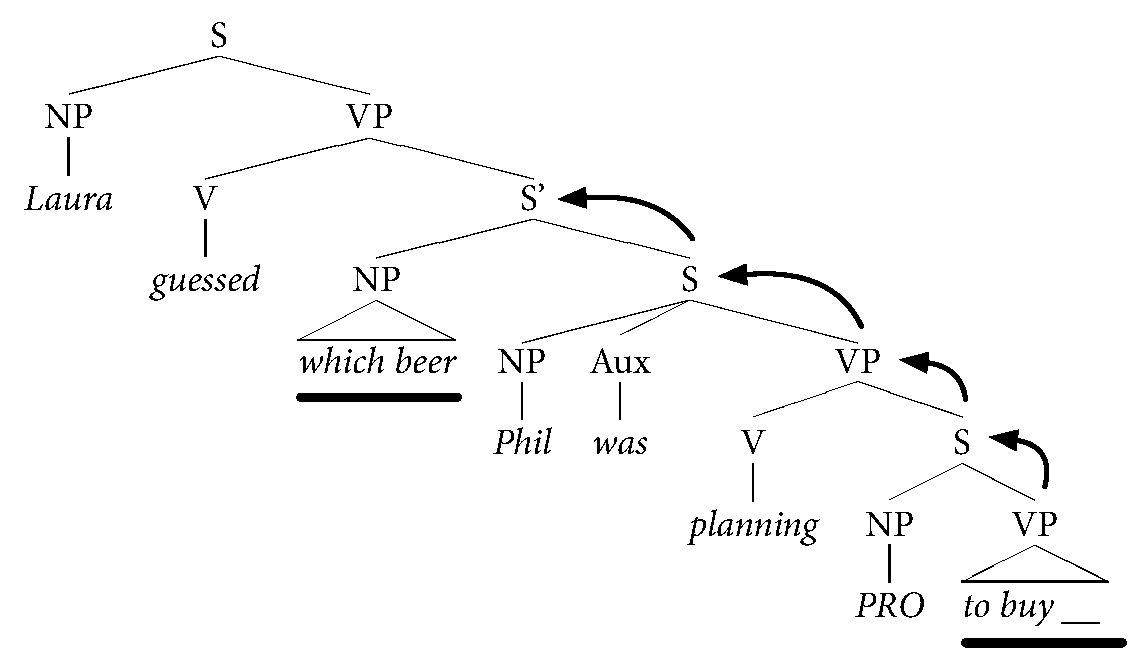
\includegraphics[width=0.5\textwidth]{structuresearch.pdf}}
  \subfloat[Cue-based search.]{\label{contentsearch}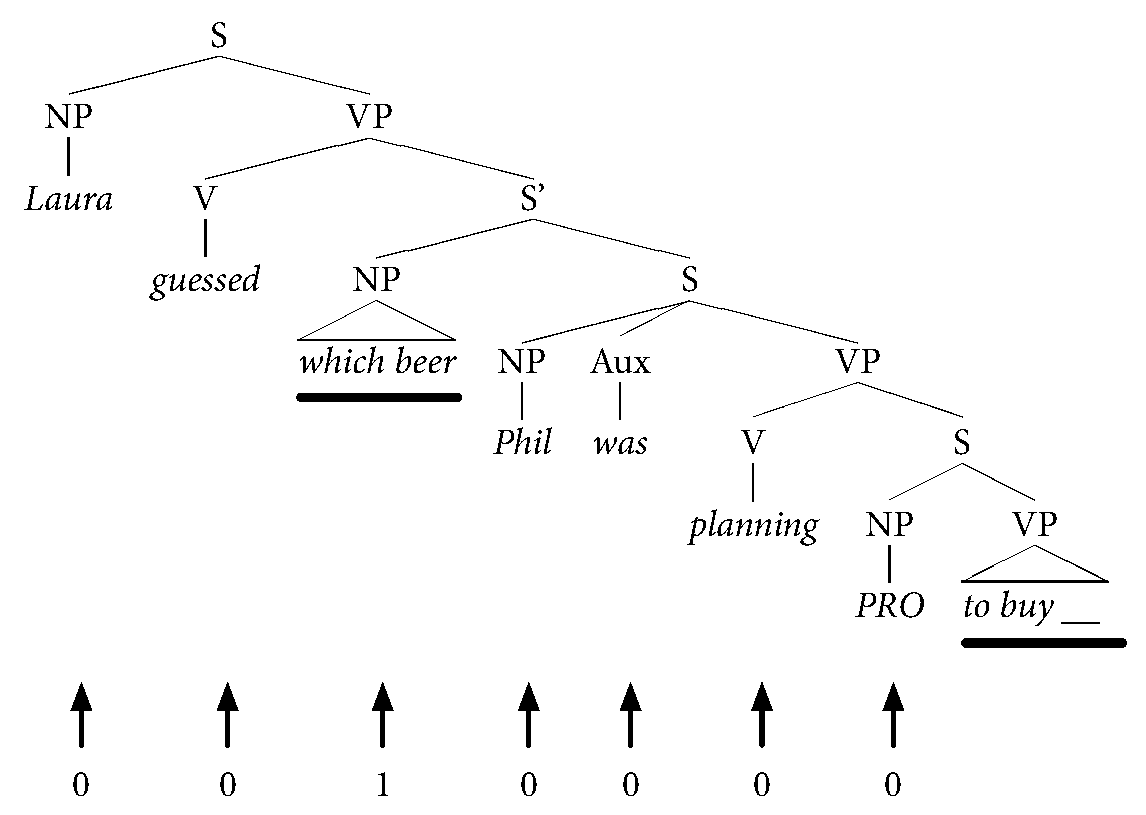
\includegraphics[width=0.5\textwidth]{contentsearch.pdf}}
  \caption{Retrieval algorithms.}
\end{figure}


\section{Constraints}

The grammar sets forth constraints on which elements can enter into dependency relations. In question is what role these constraints play in online processing. Experimental evidence indicates that there is a great deal of variability in how accurately grammatical constraints are implemented online. We owe an explanation for this variability. One dimension that seems to account for some of it is the \emph{directionality} of dependencies.

\subsection{Dependencies} 

Grammatical dependencies have two elements, which we will call the \emph{left-} and \emph{right-hand} elements, based on their position in a sentence string. Generally, one of these elements alerts the parser that a dependency exists and the second element is the one that needs to be located in order to satisfy the dependency. There are cases when the left-hand element is the one that signals that a dependency is present, as in \ref{forwards}. These are considered \emph{forwards} dependencies because the parser must look \emph{forwards} in time in order to locate the second element of the dependency. Oppositely, in a \emph{backwards} dependency, like \ref{backwards}, the right-hand element is the signal. The parser must look \emph{backwards} in time (i.e., into memory) in order to locate the second element and satisfy the dependency. It should be made clear that we describe dependencies in this way because it is useful and not because these are theoretically entrenched notions.

\exg. While he ate, John watched TV.\hspace{2.65em}\textsc{forwards dependency}\\
      {} \textsc{l-signal} {} \textsc{r}\\ \label{forwards}

\exg. John watched TV while he ate.\hspace{3em}\textsc{backwards dependency}\\
      \textsc{l} {} {} {} \textsc{r-signal}\\ \label{backwards}

We say a dependency is \emph{fallible} when processing said dependency results in actions that do not respect constraints in the grammar. Such actions include considering an ineligible element for retrieval, positing a gap in an ineligible position, or fully retrieving the incorrect element from memory. This is in contrast to a \emph{faithful} dependency. Examples of both of these types of dependency will be discussed in the coming sections.

There is evidence that the directionality of a dependency---that is, whether the signaling element comes first or second---is somewhat correlated with the fallibility of the dependency. \citet{phillips09} present evidence that forwards dependencies are more faithful that backwards dependencies. They claim that prospective, forwards search is a more robust mechanism for search than is retrieval. In the next sections I present an example of a robust forwards dependency, cataphora, and several examples of backwards dependencies with mixed fallibility profiles.

\section{Cataphora, a forwards dependency} 

One forwards-looking dependency that seems to be fairly robust against interference and to consistently respect grammatical constraints is backwards anaphora, or \emph{cataphora}. In regular anaphora, antecedents precede pronouns \ref{forwards2}. In cataphora, the arrangement is reversed.

Unlike anaphora, cataphoric dependencies are forward-looking because, in these cases, the element that signals the dependency (i.e., the pronoun) precedes the element that completes it (the antecedent), so when the signaling element is identified, a second, completing element is expected \ref{backwards2}. A cross-linguistically well-attested constraint on backwards anaphora is Binding Principle~C \citep{chomsky81}, which prevents an R-expression and a c-commanding pronoun from coreferring \ref{cat-bad}. If the parser respects Principle C online, then it should not consider R-expressions that a cataphoric pronoun c-commands as possible antecedents for that pronoun. 

\ex. While he\sub{1} ate, John\sub{1} watched TV. \label{forwards2}

\ex. John\sub{1} watched TV while he\sub{1} ate. \label{backwards2}

\ex. *He\sub{1} said that John\sub{1} saw the movie \label{cat-bad}


In a self-paced reading study, \citet{kazanina07} presented evidence that Principle C is respected in online processing. In sentences like \ref{kaz}, the authors crossed two factors: (i) whether the pronoun and the antecedent matched in gender and (ii) whether there was a c-command relation between the pronoun and its potential antecedent. The first factor was introduced to exploit the Gender Mismatch Effect, which causes a slowdown in reading time if two elements that should agree in gender do not agree. The second factor varied whether the Principle C constraint could come into effect by having the pronoun c-command the R-expression [\ref{kaz-c}, \ref{kaz-d}] or not [\ref{kaz-a}, \ref{kaz-b}]. 

The prediction was that if Principle C is respected online, then reading times at \emph{Jessica} and \emph{Russell} should not be significantly different in \ref{kaz-c} and \ref{kaz-d}, where Principle C is in effect, but should be different in \ref{kaz-a} and \ref{kaz-b}, where it is not in effect. In \ref{kaz-c} and \ref{kaz-d}, \emph{Jessica} and \emph{Russell} are ineligible antecedents for the pronoun because the pronoun c-commands them. Therefore, they should not be considered when an antecedent is being sought out as the second element in the dependency. On the other hand, Principle C is not in effect in \ref{kaz-a} and \ref{kaz-b} because there is no c-command relation between the pronoun and the antecedent. Therefore, the R-expressions are eligible antecedents of \emph{she}. Being eligible, the parser considers them when searching out an antecedent and makes them liable to the Gender Mismatch Effect. In this case, \emph{Russell} should have slower reading times than \emph{Jessica}. The results of the study hold true to this prediction, suggesting that Principle C is reflected in online processing.

\ex. \label{kaz} \a. While she was taking classes full-time, Jessica was working two jobs to pay the bills. \label{kaz-a}
     \b. While she was taking classes full-time, Russell was working two jobs to pay the bills. \label{kaz-b}
     \c. She was taking classes full-time while Jessica was working two jobs to pay the bills. \label{kaz-c}
     \d. She was taking classes full-time while Russell was working two jobs to pay the bills. \label{kaz-d}

These results show that the parser \emph{can} respect grammatical constraints online and serve as a foundation piece for ensuing studies that rely on the parser's ability to respect grammatical constraints online for their argumentation.

\section{Backward dependencies}

The standard claim is that whether the formation of a dependency that requires a retrieval into memory is fallible or not is evidence for what kind of retrieval algorithm the sentence processor uses. The argument is that if the retrieval process that searches memory is structure-guided, then dependencies that rely on structural relations for their licensing \emph{should not} be fallible; structure should lead the retrieval process to the element it is trying to retrieve. On the other hand, if the retrieval process that searches memory is cue-based, then dependencies that rely on structural relations for their licensing \emph{should} be fallible; cue-based search ignores structure and retrieves anything that matches a cue, no matter position.

The following sections discuss studies that examine different dependencies for their fallibility. 

\subsection{Agreement}

Studies looking at subject-verb agreement over a distance suggest that the parser does not always take advantage of structural cues \citep{pearlmutter99, wagers09, alcocer09}. Though both are ungrammatical due to subject-verb agreement mismatch, readers are faster to read \ref{agreement-b} than \ref{agreement-a} and more likely to judge it as acceptable. Accounts of the exact mechanism vary, but the consensus seems to be that in \ref{agreement-b}, when performing a backwards search to find the verb's subject, the parser incorrectly retrieves the plural feature on \emph{runners} and illicitly satisfies the dependency. 

\ex.  \a. The runner  who the driver see every morning always wave say say hi. \label{agreement-a}
      \b. The runners who the driver see every morning always wave say say hi. \label{agreement-b}


This could be taken as evidence for a cue-based retrieval system. Structure should be enough to guide a search from a verb to its subject, yet the fact that agreement is fallible indicates that structure is not used as a guide.

\subsection{Reflexives}

One case of faithful backwards dependency completion is reported in \citet{sturt03}. Binding Principle A \cite{chomsky81} requires that anaphors like \emph{himself} have a c-commanding antecedent in the same clause. In \ref{sturt-sents}, upon reaching the anaphor, the parser must make a retrieval into memory to find an antecedent. If Principle A is respected online, then the structurally inaccessible NP \emph{Jennifer/Jonathan} should not be considered in the search for an antecedent (there should be no reading time slowdowns at the reflexive). In \ref{sturt-sents}, the subject \emph{surgeon} is stereotypically biased towards masculine referents. There is evidence that readers are subject to this bias during online comprehension. This bias might lead readers to consider \emph{Jennifer} as the antecedent to \emph{herself} despite the fact that it is structurally inaccessible. However, \citeauthor{sturt03}'s results show that readers did not consider the matching, but structurally inaccessible intervener, providing evidence that Principle A is respected online and that retrieval is structure-guided.

\ex. \label{sturt-sents} \a. The surgeon that treated Jonathan pricked himself with a needle \label{sturt-a}
      \b. The surgeon that treated Jennifer pricked herself with a needle \label{sturt-b}
      \c. The surgeon that treated Jonathan pricked herself with a needle \label{sturt-c}
      \d. The surgeon that treated Jennifer pricked himself with a needle \label{sturt-d}


This could be taken as evidence for structure-guided search. In the case reflexives, it seems that the retrieval mechanism uses structure to locate the appropriate antecedent. This is evidenced by the fact that the intervening potential antecedent is not considered at all during retrieval.


\subsection{Negative polarity items}

Negative polarity items (like \emph{any} or \emph{ever}) are licensed by a c-commanding negative element\footnote{This is a simplification. NPIs are licensed by elements that create downward entailing contexts. The c-command requirement is a side effect of how semantic interpretation licenses such entailments.}, as in \ref{NPI-a}. NPIs are not licensed when not c-commanded by a negative element, as in \ref{NPI-b} (negative element absent) or \ref{NPI-c} (negative element not c-commanding).

\ex. \a. No professor will ever say that. \label{NPI-a}
     \b. *A professor will ever say that. \label{NPI-b}
     \c. *A professor that no student likes will ever say that. \label{NPI-c}


Studies across languages and paradigms have shown, however, that NPI licensing can be interfered upon by a linearly intervening non-c-commanding element \citep[][et seq.]{drenhaus05}. For instance, in a speeded grammaticality judgment study, \citet{xiang06} found that participants were 15--30\% more likely to judge a sentence like \ref{xiang-c} as acceptable than \ref{xiang-b}.

\ex. \a. No bills that the senator voted for will ever become law.    \label{xiang-a}
     \b. *The bills that the senators voted for will ever become law. \label{xiang-b}
     \c. *The bills that no senators voted for will ever become law.  \label{xiang-c}


The c-command relation is structural and should not be fallible if memory is searched using structure. \citet{vasishth08} have taken the fallibility of NPI licensing as evidence for cue-based retrieval, though it is not clear what the search cues in this case would be exactly. \citet{xiang09} suggest that erroneous semantic/pragmatic inferences may be to blame, not retrieval.


\subsection{Shortcomings}

Unfortunately, none of these cases are water-tight, knock-down evidence for either kind of retrieval mechanism. Agreement require that the two elements of the dependency be in the same clause. Reflexives share this feature. It is possible that elements within the same clause are specially encoded and that a cue-based algorithm takes advantage of this encoding. These studies, therefore, are not conclusive evidence for either kind of retrieval mechanism. 

Further, it is not obvious that NPI licensing requires retrieval. Licensing of this kind of dependency may rely on some semantic or pragmatic computation which makes no reference to retrieval. If this is the case, then evidence from NPI licensing is not useful evidence for determining the nature of the retrieval mechanism.

The crucial study that has not been conducted is one which features a dependency where the elements are not clausemates, where the licensing conditions are clear, and where retrieval is clearly required. The present study therefore should serve as a key piece of evidence in the debate about how memory is searched.

\section{The present study}

\subsection{Background}

In partial null subject (NS) languages, null subjects are licensed under more restricted conditions than full NS languages. \citet{holmberg09}, examining several partial NS languages, reduce the conditions under which null subjects are licensed in these languages to two: (i) when the subject is a generic pronoun corresponding to English ``one'' and (ii) when the subject is controlled by the immediately higher overt subject.

In \ref{coreference} we see what condition (ii) looks like. In \ref{coreference-a}, the pronoun \emph{he} corefers with the subject \emph{John}. In a non-null subject language, like English, the pronoun is obligatorily overt. In full and partial NS languages, the pronoun is obligatorily null. In \ref{coreference-b}, however, full and partial NS languages differ. The pronoun in this example could be null in full NS languages, but crucially, would be obligatorily overt in partial NS languages. To restate condition (ii): the NS must be c-commanded by immediately higher overt subject for the NS to be bound to that subject; an unbound NS is illicit.

\ex. \label{coreference} \a. John$_1$ said that he$_1$ bought the house \label{coreference-a}
     \b. John$_1$ said that he$_2$ bought the house \label{coreference-b}

\runinhead{The immediately higher overt subject} C-command is necessary but not sufficient to license NS coreference. It really must be the immediately higher overt c-commanding subject. In \ref{bp-ccom1-a}, we know that the NS is intended to corefer with the non-immediate c-commanding subject \emph{João} because the NP \emph{doutor} has masculine gender marking. This is ungrammatical. On the other hand, in \ref{bp-ccom1-b}, we know that the NS is intended to corefer with the immediately higher overt subject (i.e., the first c-commanding subject that is not \emph{pro}) \emph{Maria}. This is grammatical. Crucially for our goals, the null subject and antecedent subject need not be in the same clause, as \ref{bp-ccom1-b} illustrates.

\ex. \label{bp-ccom1} \ag. *João acha que Maria pensa que é rico \label{bp-ccom1-a} \\
          J. thinks that M. thinks that is rich-\textsc{masc}\\
     \bg. João acha que Maria pensa que é doutora\\
          J. thinks that M. thinks that is rich-\textsc{fem} \label{bp-ccom1-b}\\
          ``J thinks that M. thinks that he/she is a doctor''\\


In the present study, we exploit this second condition in order to test whether backwards search is sensitive to syntactic structure. It has traditionally been tacitly assumed that a backward-looking dependency search uses syntactic structure as a guide to locate the dependency in memory. Under this system, locating the appropriate c-commander is straightforward. Importantly, however, cue-based retrieval in content-addressable memory makes no reference to relational notions like c-command, making it impossible to selectively retrieve a c-commander.

In BP, therefore, the optional pronouns in \ref{bp-coref} can only be made null if they are meant to corefer with the matrix subject.

\ex. \label{bp-coref} \ag. O João$_1$ disse que (ele$_1$) tinha comprado uma casa \label{bp-coref-a} \\
                           \textsc{det} João said that he have-\textsc{pst}.\textsc{3sg} bought a house\\
                           ``João said he bought a house''
                      \bg. Os meninos$_1$ ficavam contentes quando (eles$_1$) tinham um dia de folga \label{bp-coref-b} \\
                           \textsc{det} children were happy when they have-\textsc{pst}.\textsc{3pl} a day of holiday\\
                           ``The children were happy when they had the day off''
                      \cg. A Maria$_1$ admite que (ela$_1$) não fala muito bem inglês \label{bp-coref-c} \\
                           \textsc{det} Maria admits that she \textsc{neg} speak-\textsc{prs}.\textsc{3sg} very well English\\
                           ``Maria admits that she doesn't speak English very well'' 


We can exploit this fact experimentally in order to establish the role of c-command in online dependency processing. In order to establish a c-command relation between a null subject and an overt c-commanding NP, there must be some dependence on structure in memory search. Given that the null subject and the antecedent subject are not clausemates, we can be certain that no special encoding that is triggered by clausematehood is in play. Given that the antecedent subject precedes the null subject, which is the signaling element of the dependency, making this a backwards dependency, we can be sure that a retrieval must take place. This puts us in an excellent position to determine what kind of algorithm is used in search. The only cue as to the identity of the antecedent subject available to the search algorithm is structure. If we find evidence that the parser considers the intervening, structurally inaccessible subject, this is evidence for cue-based retrieval. On the other hand, if we find evidence that no such a consideration is made, then this is evidence for structure-guided search.

\section{Pre-experiments: Verifying assumptions}

\subsection{Assumption: \citet{holmberg09}'s generalizations hold}

A major assumption of this study is that the generalizations about the constraints on BP null subjects made explicit by \citeauthor{holmberg09} hold true for the population we will be testing in Rio de Janeiro. This assumption needs to be validated. The claim that null subjects in BP are as restricted as they are is not widely known. What's more, European Portuguese (EP), a close relative of BP, is a full NS language which does not have the same NS restrictions as BP. Reviewers or readers with intuitions about EP, who may mistakenly assume that they also apply to BP, may disagree with the generalization and cast doubt upon our results. In order to get this study accepted for publication, it will be necessary to demonstrate that the effect exists in the first place.

Here we propose two ways to probe this. In \ref{bp-ccom}, the null subject has two c-commanding subjects, but only the one in the clause immediately higher to it (\emph{Maria}) should be a legal antecedent to the NS. Therefore, an adjective agreeing with the NS should agree with the immediately-higher c-commanding subject, and not any others. If participants are as sensitive to the NS constraint as \citeauthor{holmberg09} argue, then we should see much higher acceptance rates for \ref{bp-ccom-b} than \ref{bp-ccom-a}.

\ex. \label{bp-ccom} \ag. *João acha que Maria que \emph{pro} é rico \label{bp-ccom-a} \\
          J. thinks that M. thinks that is obvious that \emph{pro} is rich-\textsc{masc}\\
     \bg. João acha que Maria pensa que \emph{pro} é rica\\
          J. thinks that M. thinks that \emph{pro} is rich-\textsc{fem} \label{bp-ccom-b}\\
          ``J thinks that M. thinks that he/she is rich''


A second way to test for sensitivity would be to ask a comprehension question that probes for the identity of the antecedent of the NS. In \ref{bp-question}, we present a sentence that under a full NS language would be ambiguous. However, under a partial NS language, like BP, there should be no ambiguity: the correct answer should be \emph{Maria} because this is the subject that immediately c-commands the NS. 
  
  \exg. \label{bp-question} João acha que Maria pensa que vai chegar tarde. Q: Quem vai chegar tarde?\\
        {} J. thinks that M. thinks that will arrive late. Q: Who will arrive late?\\
        \a. *João
        \b. Maria

\subsection{Assumption: BP speakers are sensitive to number morphology}

\citet{naro00}, among others, have noted that there is some variability in number morphology production in BP speakers. If we intend to manipulate number as part of our experimental design, we should make certain that participants are sensitive to it.

In particular, some dialects of BP mark number agreement only on the pronoun, but not on the verb \ref{weird-agree-a}; only on the determiner, but not on the noun \ref{weird-agree-b} or the adjective \ref{weird-agree-c} or the verb \ref{weird-agree-f}; on the determiner and the noun, but not the adjective \ref{weird-agree-d}; on the pronoun and the noun, but not the determiner \ref{weird-agree-e}.

\ex. \ag. Eles ganha demais\\ \label{weird-agree-a}
          \textsc{3pl} win-\textsc{3sg} too.much\\
          ``They win too much''\\
     \bg. as cordona\\ \label{weird-agree-b}
          \textsc{det}-\textsc{pl} hen-\textsc{sg}\\
          ``the hens''\\
     \cg. as porta aberta\\ \label{weird-agree-c}
          \textsc{det}-\textsc{pl} door-\textsc{sg} open-\textsc{sg}\\
          ``the open doors''\\
     \dg. essas estradas nova\\ \label{weird-agree-d}
         \textsc{det}-\textsc{pl} roads-\textsc{pl} new-\textsc{sg}\\
         ``Those new roads''\\
     \eg. do meus pais\\ \label{weird-agree-e}
          of.the-\textsc{sg} my-\textsc{pl} parents-\textsc{pl}\\
          ``of my parents''\\
     \fg. As coisa tá cara\\ \label{weird-agree-f}
          \textsc{det}-\textsc{pl} thing-\textsc{sg} be-\textsc{3sg} expensive-\textsc{sg}\\
          ``Things are expensive''\\
         
Though it is likely that the population of university students we will be testing will speak Standard BP, it is nonetheless important that we verify this, especially as we wish to avoid it becoming an issue during the review process. How we will test this is still unclear.

\subsection{Administering the pre-experiments}

The pre-experiments would be administered to the participants of the main experiment after the main experiment (or perhaps as fillers to the main experiment) in order not to draw participants' attention to the experimental manipulation. The pre-experiment will allow us to quantify how sensitive each participant is to the effects we are interested in. This would give us a principled way to exclude participants who were not sensitive to the effects. Additionally, a participant's ``sensitivity score'' could later be entered as a covariate in a linear mixed-effects model.

\section{Experiment~1: Number}

Three conditions: \spacesc{Accessible Match}, \spacesc{No Match}, and \spacesc{Inaccessible Match}. The \spacesc{Accessible Match} condition should always be grammatical and the \spacesc{No Match} condition should always be ungrammatical. The \spacesc{Inaccessible Match} condition, however, should be ungrammatical, but is liable to intrusion by the subject embedded in the relative clause in the matrix subject NP.

The \spacesc{Inaccessible Match} case: Upon encountering the null subject, the parser must look for a licensor. If the parser follows structure in its search, then it should not consider the structurally inaccessible intervener NP and the sentence should be judged as ungrammatical. However, if some other search mechanism is employed---one that ignores structure to some degree---then the structurally inaccessible NP may be considered as the null subject licensor and the sentence may pass as grammatical.

\ex. \a. \spacesc{Accessible match}\\ 
     \textbf{Os meninos} que \textbf{o professor} viu no boteco da esquina disseram que era provável que \pro \textbf{fossem} chegar atrasados na sala de aula.
     \b. \spacesc{No match}\\ 
     \textbf{O menino} que \textbf{o professor} viu no boteco da esquina disse que era provável que \pro \textbf{fossem} chegar atrasados na sala de aula.
     \c. \spacesc{Inaccessible match}\\ 
     \textbf{O menino} que \textbf{os professores} viram no boteco da esquina disse que era provável que \pro \textbf{fossem} chegar atrasados na sala de aula.


An additional factor that may be worth manipulating is the number of the critical verb and the agreeing (or potentially agreeing) material above it. As agreement attraction experiments have shown, in relative clause constructions the number of the matrix subject NP can interfere with the subject-verb relation in the RC. In English, ungrammatical agreement between a singular RC subject and plural verb can be remedied somewhat by a plural main subject. In Spanish, however, there is evidence to suggest that \emph{grammatical} agreement between a singular RC subject and a singular RC verb is made worse by a plural main subject \citep{alcocer09}. This suggests that in order to rule out the possibility of agreement attraction playing a role on the ultimate reading time profile of these sentences, the complementary set of conditions should be included.

\ex. \a. \spacesc{Accessible match}\\ 
     \textbf{O menino} que \textbf{os professores} viram no boteco da esquina disse que era provável que \pro \textbf{fosse} chegar atrasado na sala de aula.
     \b. \spacesc{No match}\\ 
     \textbf{Os meninos} que \textbf{os professores} viram no boteco da esquina disseram que era provável que \pro \textbf{fosse} chegar atrasado na sala de aula.
     \c. \spacesc{Inaccessible match}\\ 
     \textbf{Os meninos} que \textbf{o professor} viu no boteco da esquina disseram que era provável que \pro \textbf{fosse} chegar atrasado na sala de aula.
     
\subsection{Predictions}

If search is entirely guided by structure, then the condition in which a number-agreeing, but structurally inaccessible NP intervenes between the verb and the subject head NP (\spacesc{Inaccessible match}) should be just as slow as a condition where neither of the subject NPs before the verb agrees with it. This should return a pattern of reading times like those in \ref{ex:structure-pred}.

\ex. \spacesc{Accessible match} $<$ \spacesc{Inaccessible match} $=$ \spacesc{No match} \label{ex:structure-pred}

If cues other than structure are used in search, then a structurally inaccessible, but number agreeing subject NP might be temporarily considered as the antecedent of the null subject. In this case, we would expect that, on average, reading times at the critical word in the \spacesc{Inaccessible match} would be somewhere between the average reading times at the same word in the \spacesc{Accessible match} condition (fastest) and the \spacesc{No match} condition (slowest). 

\ex. \spacesc{Accessible match} $<$ \spacesc{Inaccessible match} $<$ \spacesc{No match}

\subsection{Materials requirements}

Experimental stimuli will be presented to participants pseudo-randomly in a Latin square design. This entails that every participant will be presented with exactly one condition from each item set and equal amounts of each condition across the whole experimental session. The major limiting factor to take into consideration is time. No session should go over one hour. Given this constraint, Table~\ref{table:timing} shows that including the number factor, for a total of 6 conditions and 36 item sets, is feasible.

In order to get an equal number of observations for each experimental item, the total number of participants should be a multiple of the number of conditions. For instance, with 6 conditions, 6 participants would be required in order for each experimental item to have been seen once. In order to get enough statistical power to bring effects of the size typically seen in psycholinguistic experiments like this one into significance, at least 5 or 6 observations per experimental item would be necessary. In order to get a reasonable number of observations per item, we will need at least 30 subjects.

It does not seem possible to combine Experiments 1 and 2 into a single session. A second set of 30 subjects will therefore be required for this experiment.

\begin{table}[h]
  \centering
  \begin{tabular*}{\textwidth}{@{\extracolsep{\fill}}ccccccc}
  \toprule
  Conditions &  Experimental & Filler  & Total & Observations  & Est. completion\\
             &  items        & items   & items & per condition & time (minutes)\\
  \midrule
  3 & 18 & 36 & 54  & 6 & 18\\
  6 & 36 & 72 & 108 & 6 & 36\\
  \bottomrule
  \end{tabular*}
  \caption{Estimated completion time calculations. Assumes that each trial takes 20 s to complete and that a filler-to-item ratio of 2:1 is appropriate.}
  \label{table:timing}
\end{table}

\subsection{Things to consider}

Sensitivity to number marking is variable in BP. We need a measure to assess how sensitive subjects are to number marking.

\section{Experiment~2: Gender}

There seems to be wide variation in Brazilian Portuguese speakers' sensitivity to number. For this reason, it might be preferable to include a second experiment that manipulates NS-adjective gender agreement rather than subject-verb number agreement. An important difference in the analysis of Experiment 2 is that the crucial word is the adjective following the verb, not the verb itself, as in Experiment 1.

\ex. \a. \spacesc{Accessible match}\\
     \textbf{O menino} que \textbf{o professor} viu no boteco da esquina disse que era lógico que \pro estava \textbf{cansado} por que não tinha dormido muito
     \b. \spacesc{No match}\\
     \textbf{A menina} que \textbf{a professora} viu no boteco da esquina disse que era lógico que \pro estava \textbf{cansado} por que não tinha dormido muito
     \c. \spacesc{Inaccessible match}\\
     \textbf{A menina} que \textbf{o professor} viu no boteco da esquina disse que era lógico que \pro estava \textbf{cansado} por que não tinha dormido muito.

\subsection{Materials requirements}
\label{sec:gender-materials}

The materials requirements for Experiment~2 are the same as Experiment~1, except that no third factor is being considered for inclusion. There is not enough evidence that genders are processed differently to merit including gender as a factor. Nonetheless, half of the items should feature critical words with masculine gender and half with feminine gender.

\begin{table}[h]
  \centering
  \begin{tabular*}{\textwidth}{@{\extracolsep{\fill}}ccccccc}
  \toprule
  Conditions &  Experimental & Filler  & Total & Observations  & Est. completion\\
             &  items        & items   & items & per condition & time (minutes)\\
  \midrule
  3 & 18 & 36 & 54 & 6 & 18\\
  3 & 24 & 48 & 72 & 8 & 24\\
  \bottomrule
  \end{tabular*}
  \caption{Estimated completion time calculations for Experiment~2. Assumes that each trial takes 20 s to complete and that a filler-to-item ratio of 2:1 is appropriate.}
  \label{table:gender-timing}
\end{table}

Given how short this experiment is and depending on how plentiful participants are, we may opt to include 8 observations per condition instead of 6.

\section{Details (and questions)}

Here we mention some questions about the details of testing that we would appreciate some clarification on.

\runinhead{Pace of testing} We hope to be in the lab at UFRJ for about 4 weeks. The design of the studies we are proposing is dependent on the number of participants that are available. Could you advise us on what the availability of participants should be during our stay?

\runinhead{Participant eligibility} Our participants should be native speakers of Brazilian Portuguese between the ages of 18 and 35. Participants may speak languages other than Brazilian Portuguese, but not natively or at a fluent level. Participants should also have never suffered from a linguistic or neurological impairment or disability.

\runinhead{Compensation} We have heard accounts that it is not common practice in Brazil to pay participants money for their participation. We have funds in our grant that can be used for this, but we are not sure whether this is appropriate in light of normal practices in Brazil. Can you advise on what is normal practice in Brazil?

If participants are not recruited through payment, as would be normal in the US, what are the standard ways of recruiting participants in your university?

\runinhead{Pre-experiment questionnaire} In order to make sure that participants can be included in the study, each participant will be presented with a short questionnaire before every experimental session. The questionnaire will include questions about age, gender, language-impairment history, educational history, and about what languages the participant speaks and how well. Additionally, in order to account for possible dialectical differences between participants, they will be asked questions about where in Brazil they grew up and where they have lived.

\runinhead{IRB} We intend to translate the Institutional Review Board (IRB) consent form that we use at the University of Maryland into Portuguese. All participants must read and sign this form at the very beginning of each experimental session. This form states that the participants have been informed of their rights as participants. Signing it acknowledges that they are participating in the study aware of these rights and are participating of their own free will. Does the Universidade Federal do Rio de Janeiro have any consent forms that they require?

%\runinhead{Facilities} We plan on using the MIT Linger software to conduct these experiments. This software can run on any platform.
%
%\begin{itemize}
%  \item What kind of computers are available for testing?
%  \item How many are available?
%  \item In the past, we have had trouble with the timing of responses when using USB keyboards. What kind of keyboards are used in the lab?
%  \item How much lab space is available for testing?
%  \item If it becomes necessary, will we be able to test multiple participants at the same time?
%\end{itemize}


\bibliography{berimbau}
\bibliographystyle{apalike}

\end{document}
